\section{Neutrino-Nucleon interactions} \label{sec:theory}
%The next line produces an indented paragraph to start the document
 %unit.  The LaTeX defaults start most units without indentations.
\hspace{\parindent}

%%%%%%%%%%%%%%%%%%%%%%%%%%%%%%%%%%%%%%%%%%%%%%%%%%%%%%%%%%%
% Particle interactions
%%%%%%%%%%%%%%%%%%%%%%%%%%%%%%%%%%%%%%%%%%%%%%%%%%%%%%%%%%%
\subsection{Two-particle interactions}
  The differential cross section for two-particle scattering is given by
  \begin{equation}\label{eq:twobodyxsec}
    d\sigma = \frac{(2\pi)^4 |\mathcal{M}|^2}{4 \sqrt{(p_1\cdot p_2)^2 - m_1^2m_2^2}}
      \cross d\Phi_2(p_1+p_2;p_3,p_4) \,,
  \end{equation}
  where $d\Phi_2(p_1+p_2;p_3,p_4)$ is an element of two-body phase space given by
  \begin{equation}\label{eq:twobodyphase}
      d\Phi_2(p_1+p_2;p_3,p_3) = \delta^4(p_1+p_2 - p_3-p_4)
        \frac{d^3\mathbf{p}_3}{(2\pi)^3 2E_3}\frac{d^3\mathbf{p}_4}{(2\pi)^3 2E_4} \,,
  \end{equation}
  and $\mathcal{M}$ is the scattering amplitude.
  Combining Eqns.~\ref{eq:twobodyxsec}~and~\ref{eq:twobodyphase} gives
  \begin{equation}
      d\sigma = \frac{|\mathcal{M}|^2}{64\pi^2}
        \frac{\delta^4(p_1+p_2-p_3-p_4)}{E_3E_4\sqrt{(p_1\cdot p_2)^2 - m_1^2m_2^2}}
        \, d\mathbf{p}_3d\mathbf{p}_4 \,.
  \end{equation}

  The scattering amplitude is given by the matrix element of the scattering
  matrix, $S$, between the final and initial states ($\mathcal{M} =
  \mel{f}{S}{i}$).  The general form of $S$ is
  \begin{equation}
    S = \sum_{n=0}^{\inf} \frac{(-i)^n}{n!}\int\dots\int d^4x_1 \, d^4x_2 \dots d^4x_n\,
      T\{\hat{\mathcal{H}}'_I(x_1)\hat{\mathcal{H}}'_I(x_2)\dots\hat{\mathcal{H}}'_I(x_n)\} \,,
  \end{equation}
  where $\hat{\mathcal{H}}'_I(x_i)$ is the interaction Hamiltonian density. The
  matrix element can more easily be determined using Feynman calculus.

  \begin{figure}[ht]
    \centering
    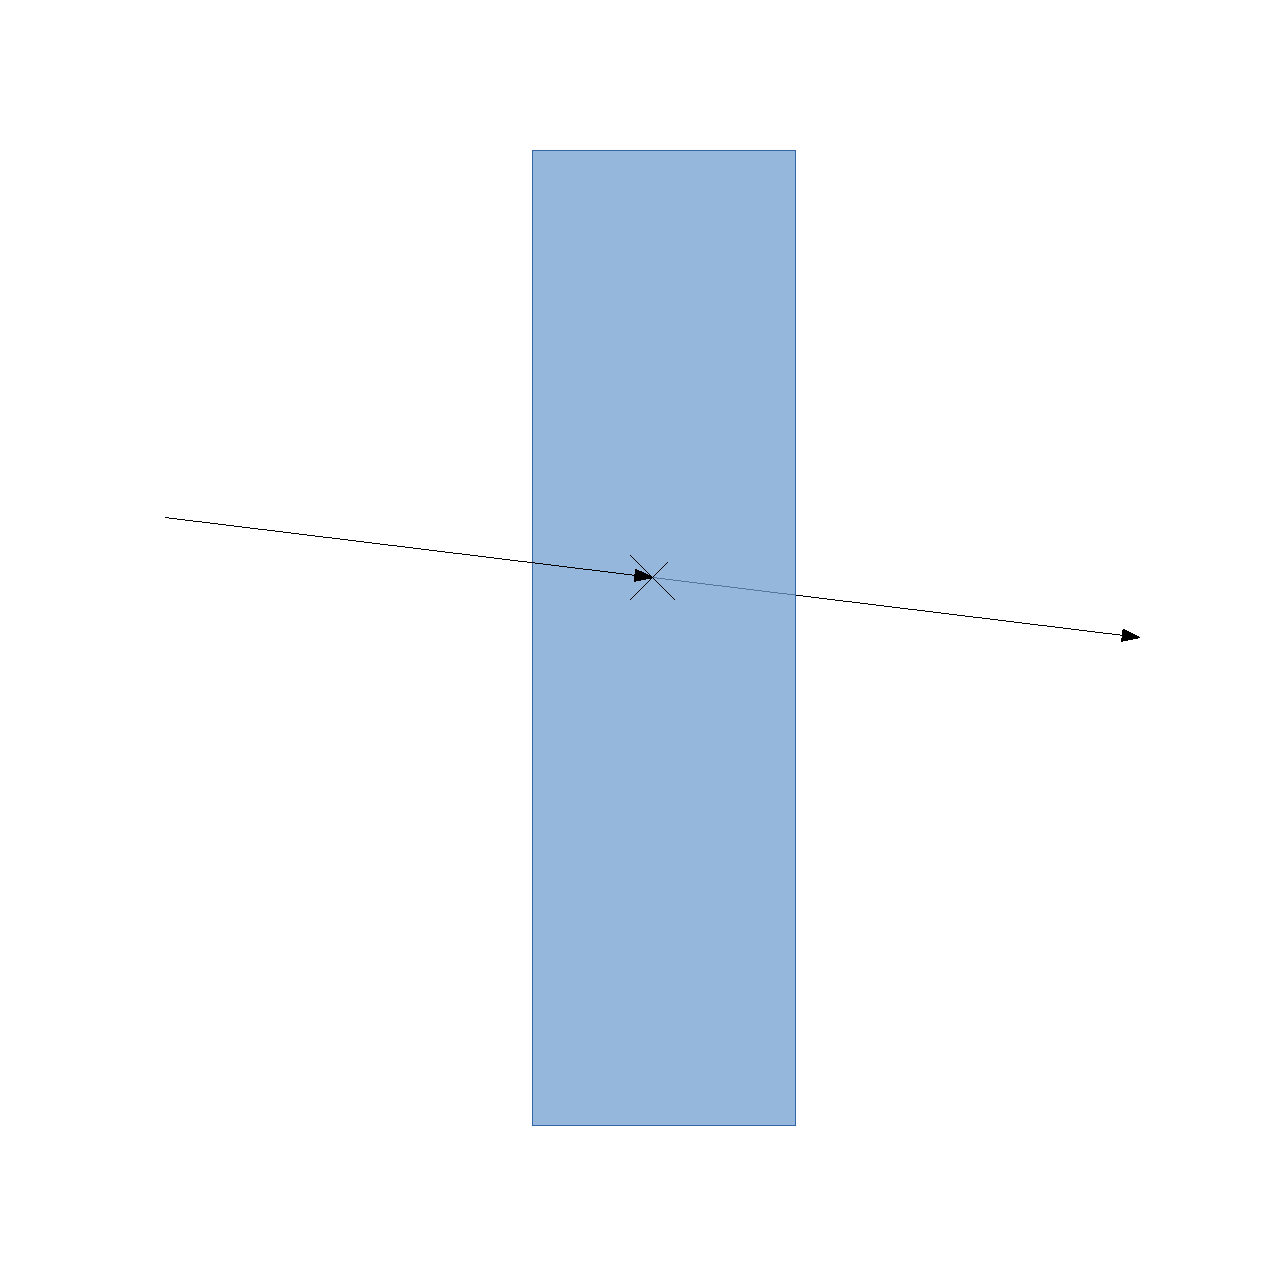
\includegraphics[angle=0,width=4in]{figures/theory/bz.pdf}
    \caption{Feynman diagram of two-fermion scattering.}
    \label{fig:feynmantwofermion}
  \end{figure}

  Figure~\ref{fig:feynmantwofermion} shows the Feynman diagram for two-fermion
  scattering. For a massive, vector-boson propagator the matrix element for
  this interaction is given by
  \begin{equation}\label{eq:genmatel}
    \mathcal{M} = \mel{f}{S}{i} = \mel{k'}{J^{\mu}(0)}{k} \frac{i}{q^2 - M_V^2}(-g_{\mu\nu} 
            + q_{\mu}q_{\nu}/M_V^2) \mel{p'}{J^{\mu}(0)}{p} \,,
  \end{equation}
  where $k$ and $k'$ initial and final four-momenta of the first fermion
  ($f_1$), $p$ and $p'$ are the initial and final four-momenta of the second
  fermion ($f_2$), $q$ is the four-momenta carried by the vector-boson
  propagator, and $M_V$ is the mass of the propagator, and $J^{\mu}$ is the
  probability current operator.


%%%%%%%%%%%%%%%%%%%%%%%%%%%%%%%%%%%%%%%%%%%%%%%%%%%%%%%%%%%
% Electroweak Interactions
%%%%%%%%%%%%%%%%%%%%%%%%%%%%%%%%%%%%%%%%%%%%%%%%%%%%%%%%%%%
\subsection{Electroweak interactions}

  The charged current, $j^{\mu}_{CC}$, which corresponds to the exchange of a
  $W^{\pm}$ boson, and the neutral current, $j^{\mu}_{NC}$, which corresponds
  to the exchange of the $Z^0$ boson are given by
  \begin{align}\label{eq:ccurrent}
      j^{\mu}_{CC} &= \sum_f \bar{\psi}_f \gamma^{\mu} (1-\gamma_5) \frac{1}{2}(\tau_1 + i\tau_2) \psi_f \\
        \label{eq:ncurrent}
      j^{\mu}_{NC} &= \sum_f \bar{\psi}_f \gamma^{\mu} (1-\gamma_5) \frac{1}{2}(\tau_3) \psi_f 
       - 2\sin^2(\theta_W) j^{\mu}_{em}
  \end{align}
  where $j^{\mu}_{em}$ is the electromagnetic current, $\psi_{f}$ are the weak
  isospin doublets, and $\tau_i$ are the Pauli matrices
  \begin{equation}
      \tau_1 = 
      \begin{pmatrix}
        0 & 1 \\
        1 & 0
      \end{pmatrix} \,,
      \hspace{5mm}
      \tau_2 = 
      \begin{pmatrix}
        0 & -i \\
        i & 0
      \end{pmatrix} \,,
      \hspace{5mm}
      \tau_3 = 
      \begin{pmatrix}
        1 & 0 \\
        0 & -1
      \end{pmatrix} \,.
  \end{equation}
  The lepton weak isospin doublets are
  \begin{equation}
    \psi_{e} = 
    \begin{pmatrix}
        \hat{\nu}_{e} \\
        \hat{e}^-
    \end{pmatrix} \,,
      \hspace{5mm}
    \psi_{\mu} = 
    \begin{pmatrix}
        \hat{\nu}_{\mu} \\
        \hat{\mu}^-
    \end{pmatrix} \,,
      \hspace{5mm}
    \psi_{\tau} = 
    \begin{pmatrix}
        \hat{\nu}_{\tau} \\
        \hat{\tau}^-
    \end{pmatrix} \,,
  \end{equation}
  and the quark weak isospin doublets are
  \begin{equation}
    \psi_{1} = 
    \begin{pmatrix}
        \hat{u} \\
        \hat{d'}
    \end{pmatrix} \,,
      \hspace{5mm}
    \psi_{2} = 
    \begin{pmatrix}
        \hat{c} \\
        \hat{s'}
    \end{pmatrix} \,,
      \hspace{5mm}
    \psi_{3} = 
    \begin{pmatrix}
        \hat{t} \\
        \hat{b'}
    \end{pmatrix} \,,
  \end{equation}
  where $d'$, $s'$, and $b'$ represent the ``mixed" states
  \begin{equation}
      \begin{pmatrix}
        \hat{d}' \\
        \hat{s}' \\
        \hat{b}'
      \end{pmatrix}
      =
      \begin{pmatrix}
          V_{ud} & V_{us} & V_{ub} \\
          V_{cd} & V_{cs} & V_{cb} \\
          V_{td} & V_{ts} & V_{tb}
      \end{pmatrix}
      \begin{pmatrix}
        \hat{d} \\
        \hat{s} \\
        \hat{b}
      \end{pmatrix}
  \end{equation}
  where $V$ is the Cabibbo-Kobayashi-Maskawa matrix. These doublets contain the
  allowed weak transitions.

  \subsubsection{The charged current}
  The combination of Pauli matrices in the charged current
  \begin{equation}
      \frac{1}{2}\tau_+ = \frac{1}{2}(\tau_1 + \tau_2) \,,
  \end{equation}
  acts as an ``isospin raising matrix" and corresponds to the exchange of a
  $W^+$ boson.
  For the leptons, this gives
  \begin{equation}
    \begin{aligned}
      j^{\mu}_{CC}(\textrm{leptons}) &= \sum_{l=e,\mu,\tau}
      \begin{pmatrix}
          \bar{\hat{\nu}}_l \\
          \bar{\hat{l}}
      \end{pmatrix}
      \gamma^{\mu}(1-\gamma_5)\frac{1}{2}
      \begin{pmatrix}
        0 & 1 \\
        0 & 0
      \end{pmatrix}
      \begin{pmatrix}
        \hat{\nu}_l \\
          \hat{l}
      \end{pmatrix} \\
      &= \sum_{l=e,\mu,\tau} \bar{\hat{\nu}}_{l} \gamma^{\mu}(1-\gamma_5)\frac{1}{2}\, \hat{l} \,,
    \end{aligned}
  \end{equation}
  and, similarly, for the quarks we get
  \begin{equation}
      j^{\mu}_{CC}(\textrm{quarks}) =
       \bar{\hat{u}}\gamma^{\mu}(1-\gamma_5)\frac{1}{2}\,\hat{d}'
       +\bar{\hat{c}}\gamma^{\mu}(1-\gamma_5)\frac{1}{2}\,\hat{s}'
       +\bar{\hat{t}}\gamma^{\mu}(1-\gamma_5)\frac{1}{2}\,\hat{b}' \,,
  \end{equation}
  with the total charged current being $j^{\mu}_{CC} =
  j^{\mu}_{CC}(\textrm{leptons}) + j^{\mu}_{CC}(\textrm{quarks})$.

  \subsubsection{The neutral current}
  In neutral current scattering, $\frac{1}{2}\tau_3$ gives the weak isospin
  which acts as a ``weak charge". The electromagnetic current is given by
  \begin{equation}
      j^{\mu}_{em} = \sum_f Q_f \bar{\hat{f}} \gamma^{\mu} \hat{f}
  \end{equation}
  where $f$ is the fermions, and $Q_f$ is the electric charge of $f$.
  So, the total neutral current is
  \begin{equation}
    \begin{aligned}
        j^{\mu}_{NC} &= \sum_{l=e,\mu,\tau} \left(\bar{\hat{\nu}}_{l}
        \gamma^{\mu}(1-\gamma_5) \frac{1}{2}\, \hat{\nu}_{l} - \bar{\hat{l}}
        \gamma^{\mu}(1-\gamma_5) \frac{1}{2}\, \hat{l} 
        +\sin^2\theta_W \bar{\hat{l}}\gamma^{\mu}\hat{l} \right) \\
        &+ \sum_{q=u,c,t} \left(\bar{\hat{q}} \gamma^{\mu}(1-\gamma_5)\frac{1}{2}\hat{q} 
        - \sin^2\theta_W \frac{2}{3} \bar{\hat{q}}\gamma^{\mu}\hat{q} \right) \\
        &+ \sum_{q=d,s,b} \left(- \bar{\hat{q}} \gamma^{\mu}(1-\gamma_5)\frac{1}{2}\hat{q} 
        + \sin^2\theta_W \frac{1}{3} \bar{\hat{q}}\gamma^{\mu}\hat{q} \right) \,.
     \end{aligned}
  \end{equation}
 
  \subsubsection{V$-$A structure}

  We can separate the currents into their vector and pseudovector, or axial
  vector, components. The terms that contain just $\gamma^{\mu}$ behave like
  vectors under a parity transformation
  \begin{equation}
    \hat{\textrm{\textbf{P}}}\hat{\psi}(\textbf{x},t)\hat{\textrm{\textbf{P}}}^{-1} \, 
      \gamma^{\mu} \, \hat{\textrm{\textbf{P}}}\hat{\psi(\textbf{x},t)}\hat{\textrm{\textbf{P}}}^{-1} 
      = - \hat{\textrm{\textbf{P}}}\hat{\psi}(-\textbf{x},t)\hat{\textrm{\textbf{P}}}^{-1} \, 
      \gamma^{\mu} \, \hat{\textrm{\textbf{P}}}\hat{\psi(-\textbf{x},t)}\hat{\textrm{\textbf{P}}}^{-1}
  \end{equation}
  where $\hat{\textrm{\textbf{P}}}$ is the parity operator
  \begin{equation}
    \textrm{\textbf{P}}: \textbf{x} \rightarrow -\textbf{x}, t \rightarrow t \,.
  \end{equation}
  The terms that contain $\gamma^{\mu}\gamma_{5}$ behave like axial vectors
  under a parity transformation
  \begin{equation}
    \hat{\textrm{\textbf{P}}}\hat{\psi}(\textbf{x},t)\hat{\textrm{\textbf{P}}}^{-1} \, 
      \gamma^{\mu}\gamma_5 \, \hat{\textrm{\textbf{P}}}\hat{\psi(\textbf{x},t)}\hat{\textrm{\textbf{P}}}^{-1} 
      = + \hat{\textrm{\textbf{P}}}\hat{\psi}(-\textbf{x},t)\hat{\textrm{\textbf{P}}}^{-1} \, 
      \gamma^{\mu}\gamma_5 \, \hat{\textrm{\textbf{P}}}\hat{\psi(-\textbf{x},t)}\hat{\textrm{\textbf{P}}}^{-1}
      \,.
  \end{equation}
  The charged current is simple
  \begin{equation}
    \begin{aligned}
    j^{\mu}_{CC} = \frac{g}{\sqrt{2}}\Bigg[&\sum_{l=e,\mu,\tau} \bar{\hat{\nu}}_l (\gamma^{\mu} 
          - \gamma^{\mu}\gamma_5)\frac{1}{2}\,\hat{l} \\
      &+ \bar{\hat{u}}(\gamma^{\mu} - \gamma^{\mu}\gamma_5)\frac{1}{2}\, \hat{d}'
      + \bar{\hat{c}}(\gamma^{\mu} - \gamma^{\mu}\gamma_5)\frac{1}{2}\, \hat{s}'
      + \bar{\hat{t}}(\gamma^{\mu} - \gamma^{\mu}\gamma_5)\frac{1}{2}\, \hat{b}' \Bigg] \,,
    \end{aligned}
  \end{equation}
  and the neutral current becomes
  \begin{equation}
    \begin{aligned}
        j^{\mu}_{NC} = \frac{g}{2\cos\theta_W} \Bigg[&\sum_{l=e,\mu,\tau} 
        \left(\bar{\hat{\nu}}_{l}(g_V^{l} \gamma^{\mu}- g_A^{l} \gamma^{\mu}\gamma_5) \hat{\nu}_{l} 
         + \bar{\hat{l}}(g_V^{l} \gamma^{\mu}- g_A^{l} \gamma^{\mu}\gamma_5)\, \hat{l} \right) \\
        &+ \sum_{q=u,d,c,s,t,b} 
         \left(- \bar{\hat{q}} (g_V^{q} \gamma^{\mu}-g_A^{q} \gamma^{\mu}\gamma_5)\hat{q} \right)\Bigg] \,.
     \end{aligned}
  \end{equation}
  where 
  \begin{equation}
    g_V^{f} = \frac{1}{2}\tau_3^{f} - 2\sin^2\theta_W Q_f \,,
    \hspace{3mm}
    g_A^{f} = \frac{1}{2}\tau_3^{f} \,.
  \end{equation}

%%%%%%%%%%%%%%%%%%%%%%%%%%%%%%%%%%%%%%%%%%%%%%%%%%%%%%%%%%%
% Nucleon Form Factors
%%%%%%%%%%%%%%%%%%%%%%%%%%%%%%%%%%%%%%%%%%%%%%%%%%%%%%%%%%%
\subsection{Nucleon form factors}

  \begin{figure}[h]
    \centering
    \begin{subfigure}{2.5in}
      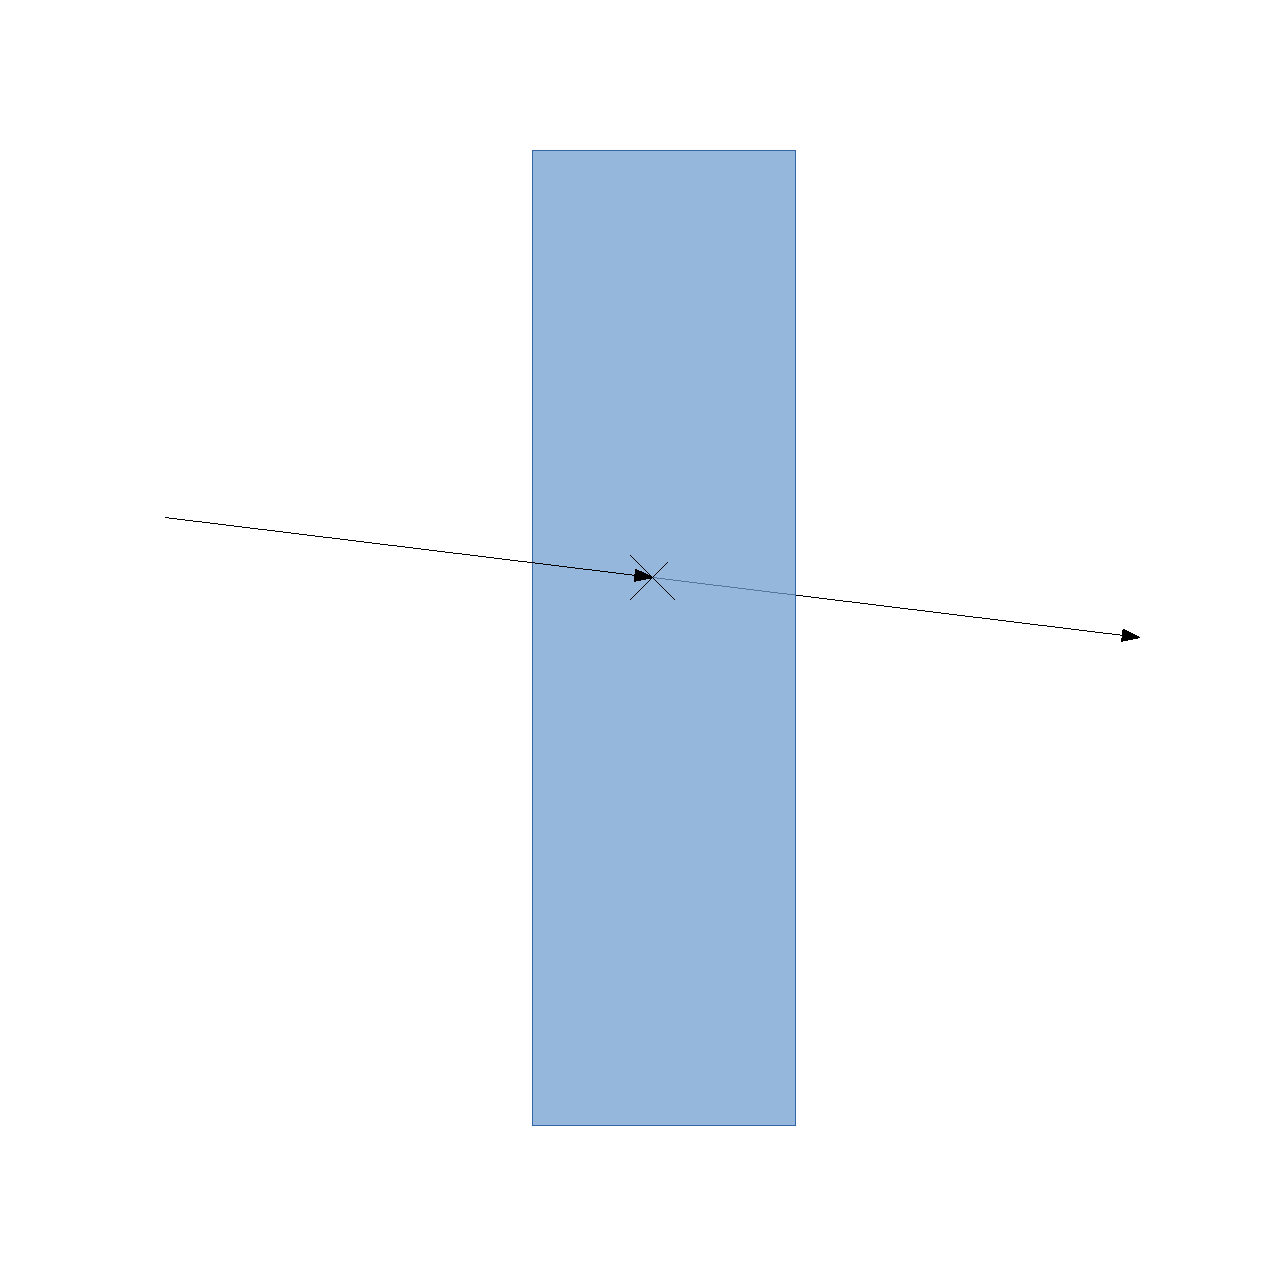
\includegraphics[angle=0,width=2.5in]{figures/theory/bz.pdf}
      \caption{Feynman diagram of neutral-current elastic lepton-nucleon
      scattering.}
      \label{fig:ncefeynman}
    \end{subfigure}
    \hspace{2pt}
    \begin{subfigure}{2.5in}
      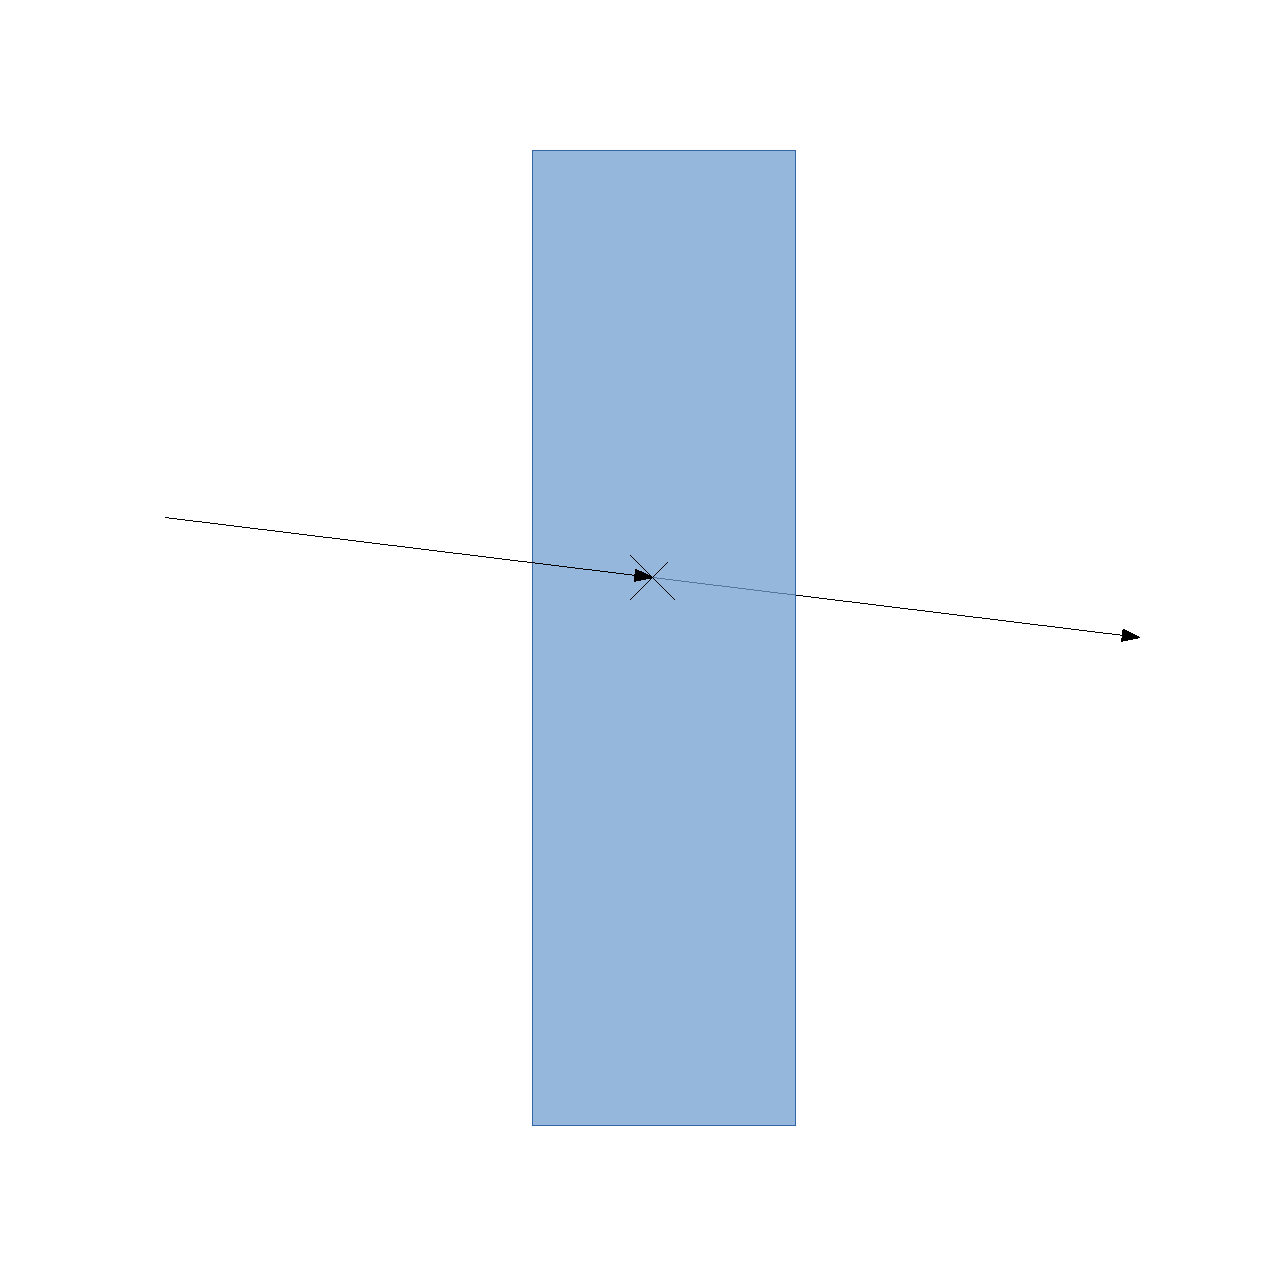
\includegraphics[angle=0,width=2.5in]{figures/theory/bz.pdf}
      \caption{Feynman diagram of charged-current elastic lepton-nucleon
      scattering.}
      \label{fig:ccqefeynman}
    \end{subfigure}
  \end{figure}

  To calculate the charged-current neutrino-nucleon scattering matrix element,
  as shown in Fig.~\ref{fig:ccqefeynman}, we need to determine the lepton CC
  matrix element, $\sideset{_{l}_}{{\nu_l}}{\mel{k'}{J^{\mu}_{CC}(0)}{k}}$, and the nucleon
  CC matrix element, $\sideset{_{\textrm{p}}}{_{\textrm{n}}}{\mel{p'}{J^{\mu}_{CC}(0)}{p}}$,
  and for neutral-current, as shown in Fig.~\ref{fig:ncefeynman}, we need the
  lepton NC matrix element, $\sideset{_{\nu_l}}{_{\nu_l}}{\mel{k'}{J^{\mu}_{NC}(0)}{k}}$, and
  the nucleon NC matrix element,
  $\sideset{_{\textrm{p}}}{_{\textrm{p}}}{\mel{p'}{J^{\mu}_{NC}(0)}{p}}$. Leptons are
  point-like particles, so their matrix elements are straight-forward
  \begin{equation}
    \begin{aligned}
      \sideset{_l}{_{\nu_l}}{\mel{k'}{J^{\mu}_{CC}(0)}{k}}
        &= -i\frac{G_F}{\sqrt{2}}u(k')(\gamma^{\mu} - \gamma^{\mu}\gamma_5)u(k) \,, \\
        \sideset{_{\nu_l}}{_{\nu_l}}{\mel{k'}{J^{\mu}_{NC}(0)}{k}}  
        &= -\frac{G_F}{\sqrt{2}}u(k')(\gamma^{\mu} - \gamma^{\mu}\gamma_5)u(k) \,.
    \end{aligned}
  \end{equation}

  \subsubsection{Nucleon matrix elements}
  Since nucleons have a finite structure, the nucleon matrix elements have a
  more complicated form. The current is corrected by form factors which
  represent the internal nucleon structure.

  If we define the vector and axial parts of the nucleon currents by
  \begin{equation}
    \begin{aligned}
    v^{\mu}_i &= \bar{\hat{\psi}}_f\, \gamma^{\mu}\frac{1}{2}\tau_i\, \hat{\psi}_f \,, \\
    a^{\mu}_i &= \bar{\hat{\psi}}_f\, \gamma^{\mu}\gamma_5\frac{1}{2}\tau_i\, \hat{\psi}_f \,,
    \end{aligned}
  \end{equation}
  where $\hat{\psi}$ are the quark doublets and $\tau_i$ are the Pauli matrices
  still, then the nucleon charged and neutral current become
  \begin{equation}
    \begin{aligned}
      j^{\mu}_{CC} &= v^{\mu}_+ - a^{\mu}_+ \,, \\
      j^{\mu}_{NC} &= v^{\mu}_3 - a^{\mu}_3 - 2\sin^2\theta_W j^{\mu}_{em;q} \,,
    \end{aligned}
  \end{equation}
  where $v^{\mu}_+ = v^{\mu}_1 + iv^{\mu}_2$ and $a^{\mu}_+ = a^{\mu}_1 +
  ia^{\mu}_2$. The nucleon matrix elements become
  \begin{equation}
    \begin{aligned}
      \sideset{_{\textrm{p}}}{_{\textrm{n}}}{\mel{p'}{J^{\mu}_{CC}}{p}} 
          &= \sideset{_{\textrm{p}}}{_{\textrm{n}}}{\mel{p'}{V^{\mu}_{+}}{p}} 
            - \sideset{_{\textrm{p}}}{_{\textrm{n}}}{\mel{p'}{A^{\mu}_{+}}{p}} \,, \\
      \sideset{_{\textrm{p}}}{_{\textrm{p}}}{\mel{p'}{J^{\mu}_{NC}}{p}} 
          &= \sideset{_{\textrm{p}}}{_{\textrm{p}}}{\mel{p'}{V^{\mu}_{3}}{p}} 
            - \sideset{_{\textrm{p}}}{_{\textrm{p}}}{\mel{p'}{A^{\mu}_{3}}{p}} 
            - \sideset{_{\textrm{p}}}{_{\textrm{p}}}{\mel{p'}{J^{\mu}_{em}}{p}} \,.
    \end{aligned}
  \end{equation}

  \subsubsection{Electric and magnetic form factors}

  It is easiest to first find an equation for $j^{\mu}_{em;q}$ in terms of the
  electric and magnetic form factors. The nucleon electromagnetic current
  should have the same vector form as the electromagnetic current for
  point-like particles. The available physical variables to construct the
  nucleon EM current are $p$, $p'$, $\gamma^{\mu}$. The most general form is
  \begin{equation}
    \Gamma^{\mu} = \gamma^{\mu}\cdot A + (p'^{\mu} + p^{\mu})\cdot B + (p'^{\mu} - p^{\mu})\cdot C \,,
  \end{equation}
  where $\Gamma^{\mu}$ is given by the equation
  $\sideset{_{\textrm{p}}}{_{\textrm{p}}}{\mel{p'}{J^{\mu}_{em}}{p}} =
  \bar{u}(p')\Gamma^{\mu}u(p)$, and $A$, $B$, and $C$ are arbitrary form factors.
  $\Gamma^{\mu}$ if constrained further by the Ward identity,
  $q_{\mu}\Gamma^{\mu} = 0$, which guarantees current conservation. The
  $\gamma^{\mu}$ and $(p'^{\mu} + p^{\mu})$ terms in $q_{\mu}\Gamma^{\mu}$ go
  to zero, but the $(p'^{\mu} - p^{\mu})$ term does not, so $C=0$. Using the Gordon
  identity~\cite{Gordon}, the general form for the nucleon EM current matrix
  element is
  \begin{equation}\label{eq:FFem}
    \sideset{_{\textrm{p}}}{_{\textrm{p}}}{\mel{p'}{J^{\mu}_{em}}{p}} =
      \bar{u}(p')\left[ \gamma^{\mu}F_1(Q^2) + \frac{i\sigma^{\mu\nu}q_{\mu}}{2M}F_2(Q^2)  \right]u(p) \,.
  \end{equation}
  The form factors $F_1$ and $F_2$ are the Dirac and Pauli form factors,
  respectively, and they are functions of $Q^2 = -q^2$. They can be transformed
  into the Sachs form factors, $G_E$ and $G_M$ by the relationships
  \begin{equation}
    G_E(Q^2) = F_1(Q^2) - \frac{Q^2}{4M^2}F_2(Q^2)\,, \hspace{5mm} G_M(Q^2) = F_1(Q^2) + F_2(Q^2) \,,
  \end{equation}
  where $Q^2 = -q^2$.  The electric form factor, $G_E$ represents the electric
  charge structure of the nucleon and the magnetic form factor, $G_M$,
  represents the magnetic structure. At the limit when $Q^2$ goes to zero, the
  Sachs form factors become the net charge and magnetic moment of the nucleon.
  \begin{equation}
    \begin{aligned}
      G_{E;p}(Q^2=0) = 1 \,,& \hspace{5mm} G_{M;p}(Q^2=0) = \mu_p \,, \\
      G_{E;n}(Q^2=0) = 0 \,,& \hspace{5mm} G_{M;n}(Q^2=0) = \mu_n \,,
    \end{aligned}
  \end{equation}
  where $\mu_p$ and $\mu_n$ are the proton and neutron magnetic moments.
 
  \subsubsection{Vector current form factors}

  The quark part of the electromagnetic current, $j^{\mu}_{em;q}$, can be
  written as
  \begin{equation}
    \begin{aligned}
      j^{\mu}_{em;q} &= \bar{\hat{\psi}}_f \, Q_f \gamma^{\mu}\, \hat{\psi}_f \\
                     &= \bar{\hat{\psi}}_f \, (\tau_3 + \frac{1}{6})\gamma^{\mu} \, \hat{\psi}_f \\
                     &= v^{\mu}_3 + v^{\mu}_0 \,,
    \end{aligned}
  \end{equation}
  where $v^{\mu}_0 = \frac{1}{6}\bar{\hat{\psi}}_f \, \gamma^{\mu}
  \hat{\psi}_f$. Now we can write the nucleon electromagnetic current matrix
  element in terms of the vector and isoscalar parts
  \begin{equation}
    \begin{aligned}
      \sideset{_{\textrm{p(n)}}}{_{\textrm{p(n)}}}{\mel{p'}{J^{\mu}_{em}}{p}} 
          &= \sideset{_{\textrm{p(n)}}}{_{\textrm{p(n)}}}{\mel{p'}{V^{\mu}_3 + V^{\mu}_0)}{p}} \\
          &= \sideset{_{\textrm{p(n)}}}{_{\textrm{p(n)}}}{\mel{p'}{V^{\mu}_3}{p}} 
           + \sideset{_{\textrm{p(n)}}}{_{\textrm{p(n)}}}{\mel{p'}{V^{\mu}_0}{p}} \,,
    \end{aligned}
  \end{equation}
  Since $V^{\mu}_3$ behaves like a vector under the charge symmetry operator and
  $V^{\mu}_0$ behaves as a scalar, the following equations are true
  \begin{equation}
    \begin{aligned}
      \sideset{_{\textrm{p}}}{_{\textrm{p}}}{\mel{p'}{V^{\mu}_3}{p}} 
        &= - \sideset{_{\textrm{n}}}{_{\textrm{n}}}{\mel{p'}{V^{\mu}_3}{p}} \,, \\
      \sideset{_{\textrm{p}}}{_{\textrm{p}}}{\mel{p'}{V^{\mu}_0}{p}} 
        &= + \sideset{_{\textrm{n}}}{_{\textrm{n}}}{\mel{p'}{V^{\mu}_0}{p}} \,. \\
    \end{aligned}
  \end{equation}
  Then
  \begin{align}\label{eq:V3em}
    \sideset{_{\textrm{p}}}{_{\textrm{p}}}{\mel{p'}{V^{\mu}_3}{p}} 
      &= \frac{1}{2} \left[\sideset{_{\textrm{p}}}{_{\textrm{p}}}{\mel{p'}{J^{\mu}_{em}}{p}} 
       - \sideset{_{\textrm{n}}}{_{\textrm{n}}}{\mel{p'}{J^{\mu}_{em}}{p}} \right] \,, \\
    \sideset{_{\textrm{p}}}{_{\textrm{p}}}{\mel{p'}{V^{\mu}_0}{p}} 
      &= \frac{1}{2} \left[\sideset{_{\textrm{p}}}{_{\textrm{p}}}{\mel{p'}{J^{\mu}_{em}}{p}} 
       + \sideset{_{\textrm{n}}}{_{\textrm{n}}}{\mel{p'}{J^{\mu}_{em}}{p}} \right] \,.
  \end{align}
  Combining equations~\ref{eq:FFem}~and~\ref{eq:V3em} gives
  \begin{equation}
    \sideset{_{\textrm{p}}}{_{\textrm{p}}}{\mel{p'}{V^{\mu}_3}{p}} 
      = \bar{u}(p') \left[\gamma^{\mu}F_1^V(Q^2) 
        + \frac{i\sigma^{\mu\nu}q_{\mu}}{2M}F_2^V(Q^2)\right] u(p) \,,
  \end{equation}
  where the vector form factors, $F_1^V$ and $F_2^V$ are defined as
  \begin{equation}
    \begin{aligned}
      F_1^V(Q^2) &= \frac{1}{2}\left( F_{1,\textrm{p}}(Q^2) - F_{1,\textrm{n}}(Q^2)\right) \,, \\
      F_2^V(Q^2) &= \frac{1}{2}\left( F_{2,\textrm{p}}(Q^2) - F_{2,\textrm{n}}(Q^2)\right)
    \end{aligned}
  \end{equation}
  The final vector currents are the ``raising" and ``lowering" vector currents,
  $V^{\mu}_{\pm}$, in the charged current.

  



  \subsubsection{Axial form factors}
    Derive the axial form factor. Discuss different axial form factor models
    (dipole...). Show that you can determine $\Delta s$. Make clear that
    this is the same $\Delta s$ from first subsubsection.

%%%%%%%%%%%%%%%%%%%%%%%%%%%%%%%%%%%%%%%%%%%%%%%%%%%%%%%%%%%
% Strangeness in the Nucleon
%%%%%%%%%%%%%%%%%%%%%%%%%%%%%%%%%%%%%%%%%%%%%%%%%%%%%%%%%%%
\subsection{Strangeness in the Nucleon} \label{sec:strangeness}

  If contributions to the nucleon from quarks heavier than the strange are
  neglected, the quark part of the charged and neutral currents can be
  separated between the light quarks and the strange quark.
  \begin{align}
    j^{\mu}_{CC}(\textrm{quarks}) &= \bar{\hat{N}}(\gamma^{\mu} 
                - \gamma^{\mu}\gamma_5)\frac{1}{2}\tau_{\pm}\hat{N} \,, \\
    j^{\mu}_{NC}(\textrm{quarks}) &= \bar{\hat{N}}(\gamma^{\mu} - \gamma^{\mu}\gamma_5)\frac{1}{2}\tau_3\hat{N} 
                - \bar{\hat{s}}(\gamma^{\mu} - \gamma^{\mu}\gamma_5)\frac{1}{2}\tau_3\hat{s} \,.
  \end{align}

  %%% starting text %%%
  From Alberico, starting with 2.3: \\
  It's convenient to separate the contributions from the light ($u,d$) and
  heavy ($s,c,...$) quarks. We get
  \[
    \j_{\alpha}^{NC;q} = v_{\alpha}^3 - a_{\alpha}^3 - \frac{1}{2}(v_{\alpha}^s - a_{\alpha}^s) - 2\mathrm{sin}^2\theta_W j_{\alpha}^{em} \,,
  \]
  where we define
  \begin{align*}
      v_{\alpha}^3 &= \bar{u}\gamma_{\alpha}\frac{1}{2}u - \bar{d}\gamma_{\alpha}\frac{1}{2}d \equiv \bar{N} \gamma_{\alpha}\frac{1}{2}\tau_3 N \\
      a_{\alpha}^3 &= \bar{u}\gamma_{\alpha}\gamma_5\frac{1}{2}u - \bar{d}\gamma_{\alpha}\gamma_5\frac{1}{2}d \equiv \bar{N} \gamma_{\alpha}\gamma_5\frac{1}{2}\tau_3 N \,.
  \end{align*}
  where $N = \left(\begin{matrix}{u}\\{d}\end{matrix} \right)$ is the isotopic
  SU(2) group doublet and the currents $v_{\alpha}^3$ and $a_{\alpha}^3$
  are the third components of the isovectors
  \begin{align*}
      v_{\alpha}^i &= \bar{N} \gamma_{\alpha}\frac{1}{2}\tau^i N \\
      a_{\alpha}^i &= \bar{N} \gamma_{\alpha}\gamma_5\frac{1}{2}\tau^i N \,.
  \end{align*}
  On the other hand, $v_{\alpha}^s$ and $a_{\alpha}^s$ are isoscalars. They
  represent the heavier quark contirbution to $j_{\alpha}^{NC;q}$. If we only
  include the strange quark, we have
  \begin{align*}
      v_{\alpha}^s &= \bar{s}\gamma_{\alpha}s \\
      a_{\alpha}^s &= \bar{s}\gamma_{\alpha}\gamma_5 s \,.
  \end{align*}
  The quark part of the electromagnetic current is
  \[
    j_{\alpha}^{em;q} = \sum_{q=u,d,...} e_q\bar{q} \gamma_{\alpha}q \,,
  \]
  which we can also separate between light and heavy contributions
  \[
    j_{\alpha}^{em;q} = v_{\alpha}^3 + v_{\alpha}^0 \,.
  \]
  where $v_{\alpha}^0$ is the isoscalar current which is given by
  \[
    v_{\alpha}^0 = \frac{1}{6}\bar{N}\gamma_{\alpha}N + \left(-\frac{1}{3}\right)\bar{s}\gamma_{\alpha}s \,,
  \]
  if we ignore charm and up.

  %%% ending text %%%

%%%%%%%%%%%%%%%%%%%%%%%%%%%%%%%%%%%%%%%%%%%%%%%%%%%%%%%%%%%
% Spin Structure of Nucleons
%%%%%%%%%%%%%%%%%%%%%%%%%%%%%%%%%%%%%%%%%%%%%%%%%%%%%%%%%%%
\subsection{The Spin Structure of Nucleons} \label{sec:nuctheory}
  Proton spin: \\
  --- spin vector $s_{\mu}$ from forward matrix element of axial vector current \\
  --- derive axial charges \\
  From Bass 1.1 (need to fill in with Peskin): \\
  Forward matrix element of the axial current vector (derive from peskin):
  \[
      2Ms_{\mu} = <p,s|\bar{\psi}\gamma_{\mu} \gamma_{5} \psi|p,s>
  \]
  where $s_{\mu}$ is the proton's spin vector, $\psi$ is the proton field
  vector and $M$ is the proton mass. The quark axial charges measure
  information about the quark ``spin content".
  \[
    2Ms_{\mu}\Delta q = <p,s| \bar{q}\gamma_{\mu}\gamma_{5}q|p,s> \,,
  \]
  where $q$ is the quark field operator and $\Delta q$ is the quark
  flavor-dependent axial charge, $\Delta u$, $\Delta d$, or $\Delta s$. The
  isovector, SU(3) octet, and flavor-singlet axial charges, $g_A^{(3)}$,
  $g_A^{(8)}$, and $g_A^{(0)}$, respectively, can be written as linear
  combinations of the quark axial charges (derive from Peskin)
  \begin{align}
      g_A^{(3)} &= \Delta u - \Delta d \\
      g_A^{(8)} &= \Delta u + \Delta d - 2\Delta s \\
      g_A^{(0)} &= \Delta u + \Delta d + \Delta s \,.
  \end{align}
  Can be interpreted semi-classically as amount of spin carried by quarks and
  antiquarks of flavor $q$.

  --- expectation of axial charges from non-relativistic quark model

%%%%%%%%%%%%%%%%%%%%%%%%%%%%%%%%%%%%%%%%%%%%%%%%%%%%%%%%%%%
% Neutrino-proton elastic cross section
%%%%%%%%%%%%%%%%%%%%%%%%%%%%%%%%%%%%%%%%%%%%%%%%%%%%%%%%%%%
\subsection{Neutrino-proton elastic cross section}\label{sec:probe}
  \subsubsection{Cross section model}

  \subsubsection{Previous measurements}
    E734

%This is the end of nu-N cross sections section
